\subsection{Cohort Demographics}
\label{sec:demographics}

For demographic extraction, we used an LLM-based query to retrieve age, sex, and ethnicity to characterize the demographic composition of the corpus. The prompt specified that age be reported in years, sex as Male, Female, a custom string, or Not Specified, and ethnicity according to U.S. Census categories or as Not Specified.

\subsection{LLM Prompt to Extract Demographics from PMOA Case Reports}
\label{apd:demographics-prompt}

\rebuttal{The prompt below is reproduced verbatim for reproducibility. Its outputs are described in the manuscript as LLM-extracted sex descriptors and LLM-mapped ethnicity categories, not as verified biological or self-identified attributes.}

\begin{tcolorbox}[
  colback=gray!5,
  colframe=gray!100,
  title={Prompt},
  boxrule=2pt,
  enhanced,
  breakable,                % <-- allows page breaks; starts here even if long
  before skip=8pt,          % spacing above (optional)
  after skip=8pt,           % spacing below (optional)
  pad at break*=2mm,        % padding at page break (optional)
  fontupper=\scriptsize,
  title after break={{Prompt}} % optional continuation note
]
You are an expert clinician. Extract the following demographic information from the case report: (1) age at case presentation, (2) sex (biologic sex at birth), and (3) ethnicity.  Report the age in years.  Report the sex as Male, Female, otherwise as a custom string, or Not Specified.  Report ethnicity as according to the US Census, otherwise as Not Specified.  For example, here is the case report.\\

\textcolor{teal}{\texttt{An 18-year-old male was admitted to the hospital with a 3-day history of fever and rash. Four weeks ago, he was diagnosed with acne and received the treatment with minocycline, 100 mg daily, for 3 weeks. With increased WBC count, eosinophilia, and systemic involvement, this patient was diagnosed with DRESS syndrome. The fever and rash persisted through admission, and diffuse erythematous or maculopapular eruption with pruritus was present. One day later the patient was discharged.}}\\

% \noindent
Then the demographic extraction should be:\\
\texttt{18 | Male | Not Specified} \\
 
Report the demographics with the three columns separated by a pipe '|' as a bar-separated row as above.
\end{tcolorbox}

Our analysis shows a median age of 47 years, with age distribution peaks at 5-year intervals, indicating rounding in clinical reporting (Figure \ref{fig:demo}). The gender distribution is balanced (52\% male, 47\% female, and 1\% with unspecified gender.) Most case reports (89\%) do not specify the patient's ethnicity. When ethnicity is specified, White/Caucasian (5\%) and Asian (3\%) are the most common, followed by African (1\%) and Other (2\%). Compared to U.S. population demographics, Asian patients are overrepresented, likely due to the international scope of PubMed publications.

\begin{figure}[!htbp]
  \centering
  \begin{minipage}[t]{0.49\linewidth}\vspace{0pt}
    \centering
    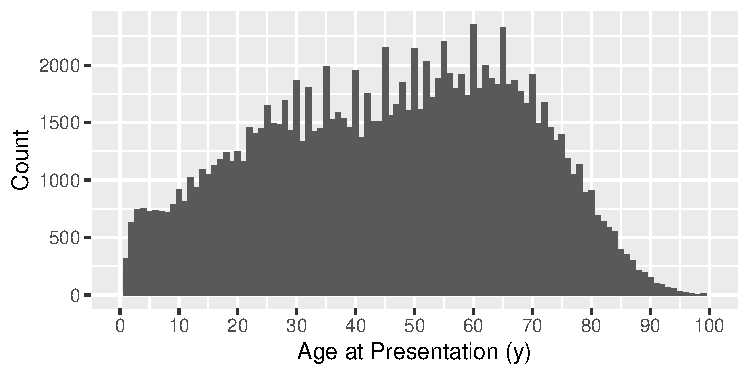
\includegraphics[width=\linewidth]{Scientific_data/Plots_tables/125k_age.pdf}
  \end{minipage}\hfill
  \begin{minipage}[t]{0.49\linewidth}\vspace{0pt}
    \centering
    \scriptsize
    \begin{tabular}{l r}
      \toprule
      \textbf{Characteristic} & \textbf{Percent (\%)}\\
      \midrule
      \multicolumn{2}{l}{\textbf{Sex}}\\
      \quad Male & 52\\
      \quad Female & 47\\
      \quad Not Specified & 1\\
      \midrule
      \multicolumn{2}{l}{\textbf{Ethnicity}}\\
      \quad White/Caucasian & 5\\
      \quad Asian & 3\\
      \quad African & 1\\
      \quad Other & 2\\
      \quad Not Specified & 89\\
      \bottomrule
    \end{tabular}
  \end{minipage}
  \caption{\rebuttal{Age distribution and LLM-mapped/extracted demographic descriptors for 124{,}349 PMOA-TTS case reports.}}
  \label{fig:demo}
  \vspace{-7.5mm}
\end{figure}


%%%%%%%%%%%%%%%%%%%%%%%%%%%%%%%%%%%%%%%%%%%%%%%%
%%%%%%%%%%%%%%%%%%%%%%%%%%%%%%%%%%%%%%%%%%%%%%%%

\subsection{Descriptive Statistics}

The textual time series in the dataset exhibit substantial variability in sequence length. 
On average, each TTS contains $\sim46$ timesteps, with 50\% of sequences comprising between 33 and 57 timesteps (Figure~\ref{fig:tts_stats}). 
The distribution of time series lengths is right-skewed, with a small number of exceptionally long sequences extending beyond $1,000$ timesteps. 
Each clinical event spans an average of 3.6 words (26.1 characters), with most events being concise, typically ranging between two and five words. 
Examples of concise events include those shown in Figure~\ref{fig:tts_stats}, while a long event example ($\geq15$ words) is provided as follows: ``\textcolor{black}{\texttt{histologic examination showed that the mass was mainly composed of fairly uniform, polygonal chief cells}}''.

The temporal coverage of individual case reports also varies widely. 
The average case duration is 415.9 days, with a median of 104.0 days. 
Half of all cases span between 28 and 391 days, and the 99th percentile extends to $4380$ days (12 years), corresponding to the longest 1\% of cases. 
On average, 77.6\% of events share timestamps with other events, indicating frequent temporal co-occurrence. 
Across all case reports, the median uniqueness ratio of event timestamps is 0.14, suggesting that multiple events are often documented at the same time point which is a pattern commonly observed for many types of measurements when recorded.
Around 17\% of all events have a negative timestamp, referring to historical events that occurred prior to the admission event in each case report's timeline.  
These statistics describe the overall temporal scope and composition of the dataset, summarizing the variability and density of clinical event sequences across case reports.

\begin{figure}[h!]
    \centering
    \begin{minipage}{0.48\textwidth}
        \centering
        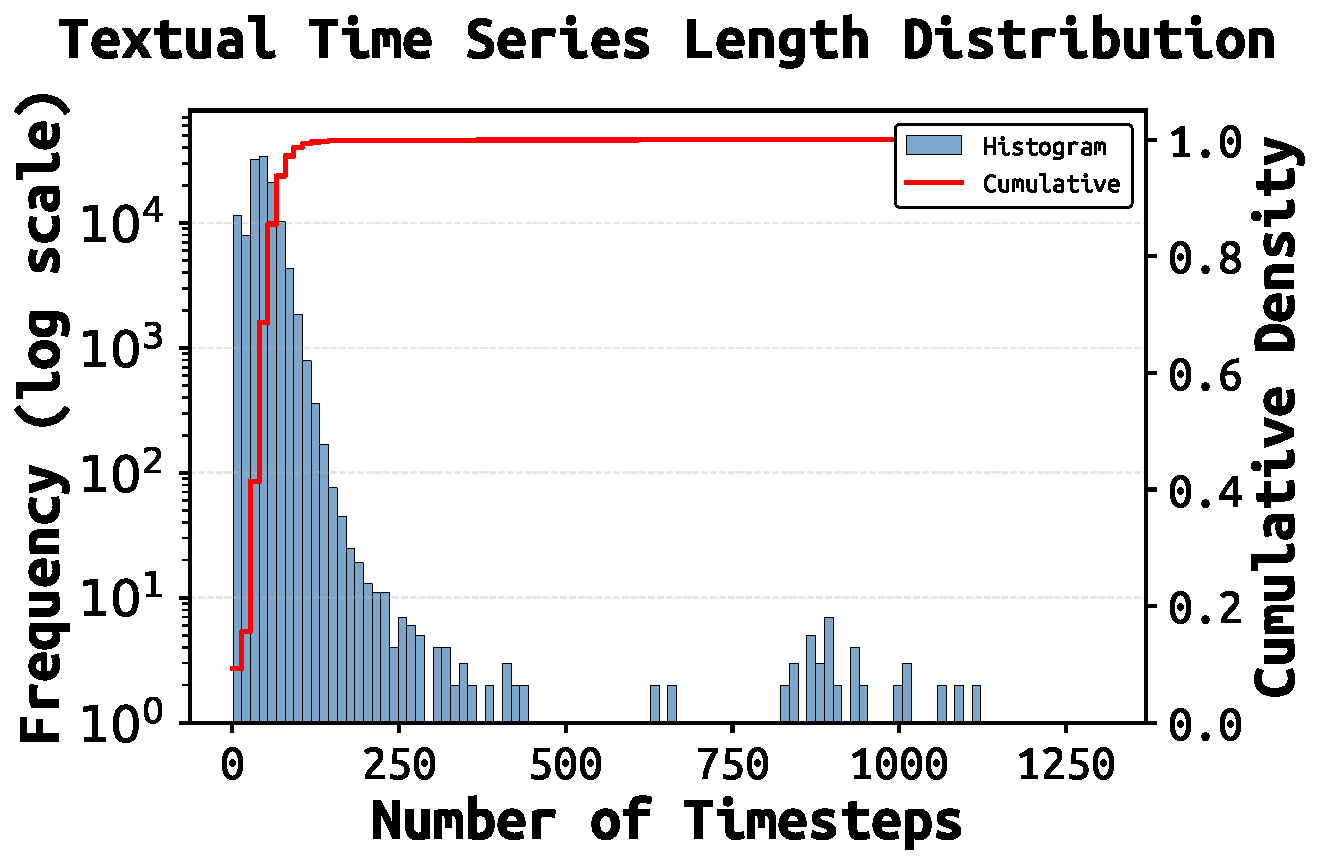
\includegraphics[width=\linewidth]{Plots_tables/tts_length_distribution.pdf}
        \caption*{(a) Distribution of time series lengths (in timesteps) across the dataset.}
    \end{minipage}\hfill
    \begin{minipage}{0.48\textwidth}
        \centering
        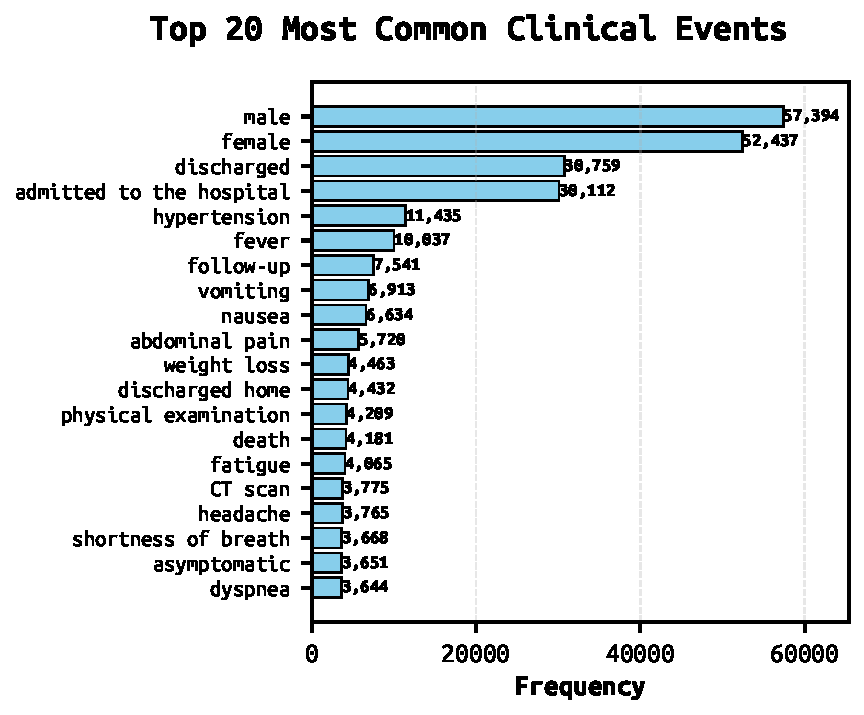
\includegraphics[width=\linewidth]{Plots_tables/top_20_common_events.pdf}
        \caption*{(b) Most frequently occurring events across all case reports. \textcolor{red}{Jeremy: Not sure why the male/female count sums to about 110k, from a cohort of 124k.}}
    \end{minipage}
    \caption{Overview of textual time series characteristics in the dataset.}
    \label{fig:tts_stats}
\end{figure}

%%%%%%%%%%%%%%%%%%%%%%%%%%%%%%%%%%%%%%%%%%%%%%%%
%%%%%%%%%%%%%%%%%%%%%%%%%%%%%%%%%%%%%%%%%%%%%%%%

\subsection{Diagnosis Distribution Analysis}

Additionally, we prompted the LLM to act as an expert physician and list patient-specific diagnoses from the report, distinguishing true diagnoses (e.g., “acne,” “DRESS syndrome”) from general clinical findings (e.g., “rash,” “leukocytosis”). The prompt instructed the model to list the primary diagnosis first, include one diagnosis per line, and omit explanatory text (full prompt shown below). 
\textcolor{red}{Jeremy: Vague: what is a "true diagnosis"? Identification or conclusion about the presences of a diagnosis rather than an isolated clinical findings?}

\subsection{LLM Prompt to Extract List of Diagnoses from PMOA Case Reports}
\label{apd:diagnosis-prompt}
\begin{tcolorbox}[
  colback=gray!5,
  colframe=gray!100,
  title=LLM prompt to extract list of diagnoses from PMOA case reports,
  boxrule=2pt,
  enhanced,
  breakable,                % <-- allows page breaks; starts here even if long
  before skip=8pt,          % spacing above (optional)
  after skip=8pt,           % spacing below (optional)
  pad at break*=2mm,        % padding at page break (optional)
  fontupper=\scriptsize,
  title after break={Prompt} % optional continuation note
]
\textcolor{teal}{\texttt{An 18-year-old male was admitted to the hospital with a 3-day history of fever and rash. Four weeks ago, he was diagnosed with acne and received the treatment with minocycline, 100 mg daily, for 3 weeks. With increased WBC count, eosinophilia, and systemic involvement, this patient was diagnosed with DRESS syndrome. The fever and rash persisted through admission and diffuse erythematous or maculopapular eruption with pruritus was present. One day later the patient was discharged.}} \\

Then the output should look like:\\
    \texttt{acne} \\
    \texttt{DRESS syndrome} \\

Rash, leukocytosis, and other findings are not diseases so they are omitted, while acne and DRESS syndrome were both diagnosed, so they are included. Output a list of diagnoses (one per line) from the following case. Place the primary diagnosis first. Include only the list and nothing else.

\end{tcolorbox}

%*******************************
\begin{figure}[!htbp]
    % \vspace{-5pt}
    \centering
    \quad
    \begin{subfigure}[t]{0.33\textwidth}
        \centering
        \raisebox{40pt}{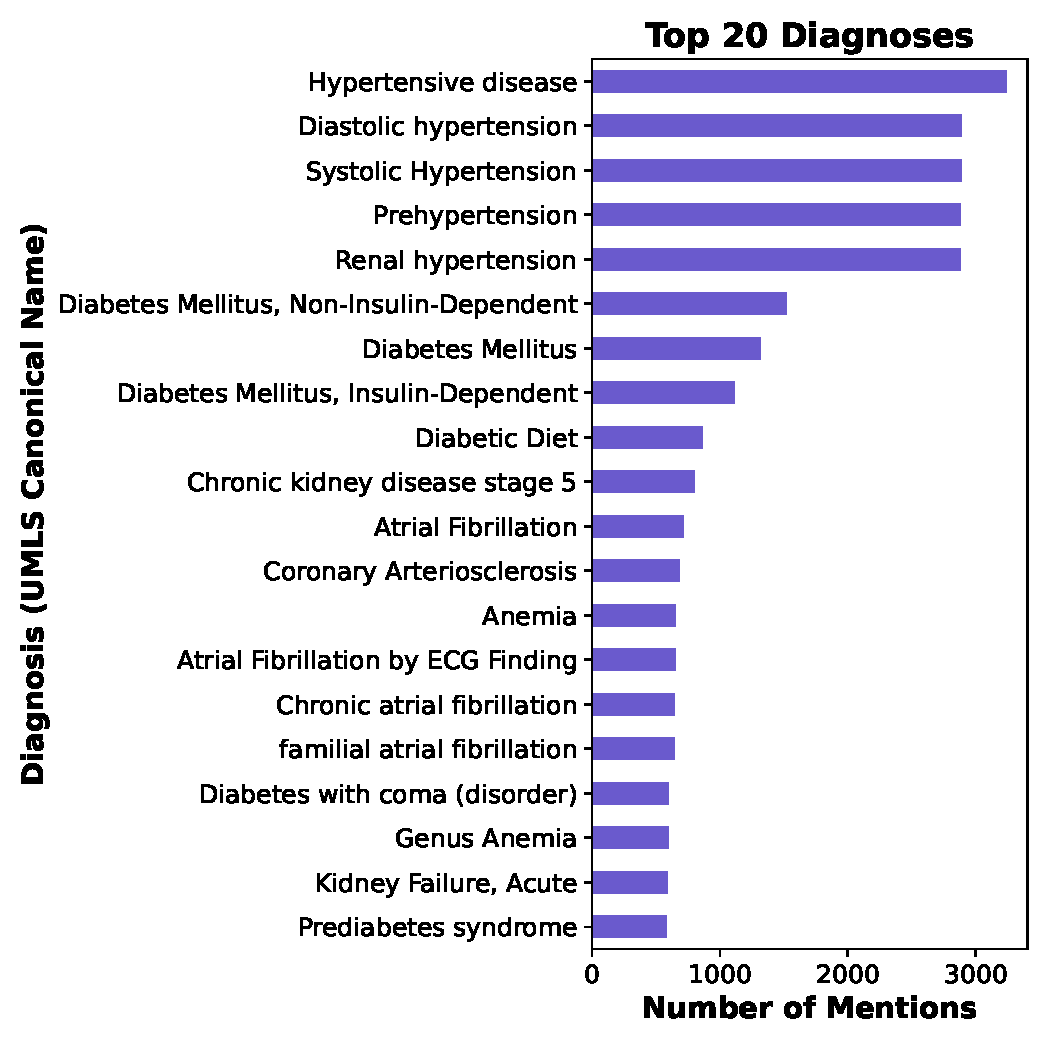
\includegraphics[width=0.99\linewidth]{Plots_tables/top_diagnoses_umls.pdf}}
        \caption{Most Frequent Diagnoses in PMOA-TTS}
        \label{fig:top_diagnoses}
    \end{subfigure}
    \hfill
    \begin{subfigure}[t]{0.6\textwidth}
        \centering
        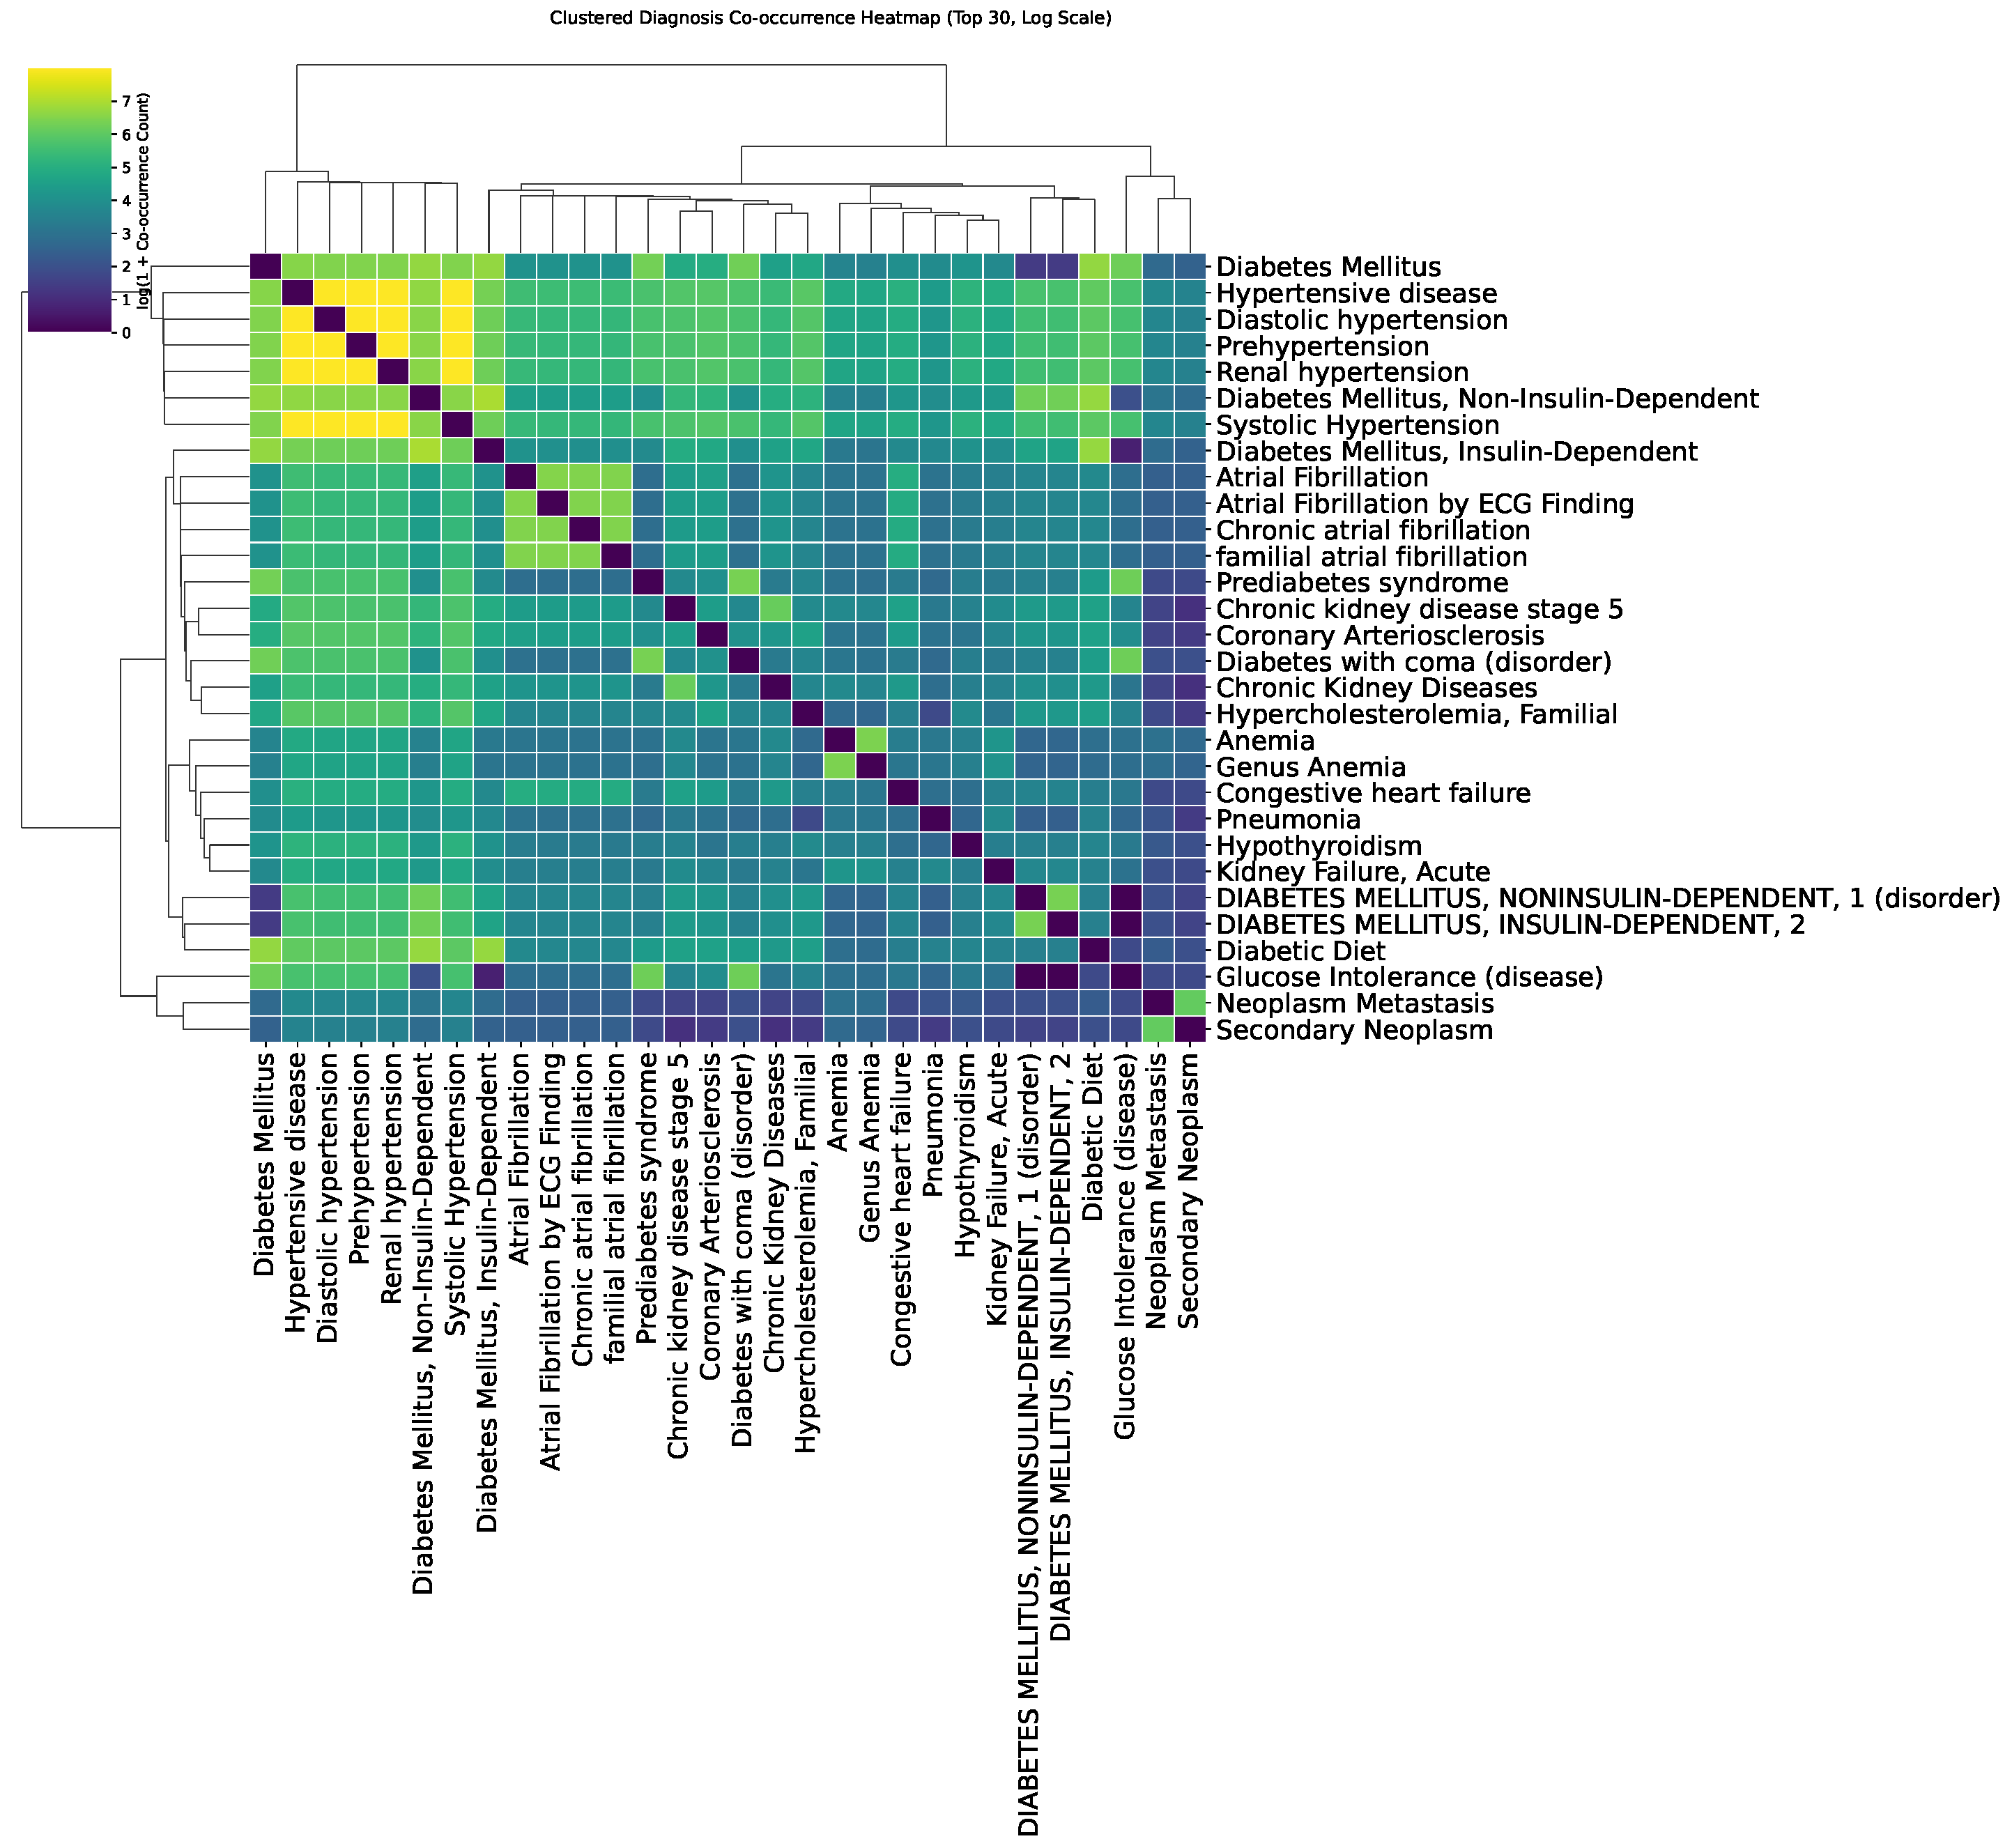
\includegraphics[width=0.99\linewidth]{Plots_tables/clustered_cooccurrence_heatmap_top30.pdf}
        \caption{Diagnoses Co-occurrence Heatmap in PMOA-TTS}
        \label{fig:diagnosis_cooccurrence}
        % \caption{}
    \end{subfigure}
    \caption{Co-occurrence Patterns and Frequency of Diagnoses in Clinical Case Reports. 
    The left panel shows the top 20 most frequently mentioned diagnoses, using UMLS canonical names, across clinical case reports. Cardiovascular and metabolic conditions such as hypertension, diabetes mellitus, and chronic kidney disease dominate the list. The right panel is a heatmap with hierarchical clustering, visualizing pairwise co-occurrence patterns (log-transformed counts) among diagnoses. Off-diagonal values reveal common comorbidity patterns in our PMOA-TTS. Clustering reveals distinct groups of frequently co-mentioned conditions, such as cardiovascular disorders and diabetes-related terms. 
    % \textcolor{red}{Shariar: Need to increase font size for better visibility}
    }
    \label{fig:diagnoses}
    \vspace{-10pt}
\end{figure}
%*******************************

%%%%%%%%%%%%%%%%%%%%%%%%%
% To assess the medical coverage of our corpus, we analyzed the diagnoses extracted through this LLM-based method, as detailed in Appendix~\ref{apd:umls_mapping}. 

\subsubsection{UMLS Mapping for Diagnosis Standardization}

To standardize the diagnoses extracted by LLMs from the case reports, we mapped the free-text diagnoses to concepts in the Unified Medical Language System (UMLS). 
This process involved the following steps:

\begin{enumerate}
    \item \textbf{Initial Extraction}: For each case report, we prompted the LLM to extract diagnoses. 
    This yielded a list of free-text diagnoses for each case report.
    \item \textbf{Entity Linking}: We used ScispaCy's entity linker model 
    \texttt{(en\_core\_sci\_lg)} with the UMLS knowledge base to map each extracted diagnosis to corresponding UMLS Concept Unique Identifiers (CUIs). 
    The entity linker identifies potential UMLS concepts and ranks them based on contextual relevance.
    \item \textbf{Filtering and Disambiguation}: For each diagnosis, we:
    \begin{itemize}
       \item Retained only mappings with a confidence score above 0.85
       \item When multiple CUIs were identified for a single diagnosis, selected the highest-ranked mapping
    \end{itemize}
    \item \textbf{Concept Normalization}: After mapping to CUIs, we:
\begin{itemize}
   \item Retrieved the canonical names from UMLS Metathesaurus
   % \item Applied semantic type filtering to ensure mapped concepts were of types relevant to diagnoses (e.g., "Disease or Syndrome", "Pathologic Function", "Mental or Behavioral Dysfunction")
   % \item Grouped synonym concepts where appropriate to reduce redundancy
\end{itemize}
\end{enumerate}

This mapping process allowed us to standardize the diverse expressions of diagnoses extracted by LLMs into a consistent terminology system, enabling more reliable frequency analysis and co-occurrence patterns. 
\textcolor{red}{Jeremy: Quantify the mapping success rate. Any effects of confidence score or justification for threshold?}

%%%%%%%%%%%%%%%
\subsubsection{Co-occurrence Patterns and Frequency of Diagnoses}
Figure~\ref{fig:top_diagnoses} shows the 20 most frequent diagnoses, demonstrating the broad clinical scope of the dataset (\textcolor{red}{Jeremy: Not at all, rather it just shows capture of modal diagnoses rather than broad coverage.}). Hypertensive disorders, including hypertensive disease, diastolic and systolic hypertension, prehypertension, and renal hypertension, are the most common, followed by diabetes mellitus and its subtypes.

This distribution aligns with the prevalence of chronic conditions typically seen in clinical practice, particularly cardiovascular, metabolic, and renal disorders, and matches the corpus’s demographic profile, with a median patient age of 45 years—an age group commonly affected by these conditions.

We also examined diagnosis co-occurrence patterns using a clustered heatmap (Figure~\ref{fig:diagnosis_cooccurrence}), revealing strong groupings of related conditions. Notably, hypertensive spectrum disorders and diabetes variants cluster together, reflecting well-established clinical links, such as those between diabetes and chronic kidney disease, or atrial fibrillation and hypertension.

This analysis highlights the diverse range of medical conditions in the PMOA-TTS corpus and demonstrates its suitability for clinical prediction tasks across multiple disease domains.


